\documentclass[a4paper,12pt]{article} 
\usepackage{enumitem}
\usepackage{color}
\usepackage{graphicx}
\usepackage{float}
\usepackage{minted}
\usepackage{hyperref}
\usepackage[parfill]{parskip}

% End loading packages

\newcommand{\bck}{
    \textbackslash
}
\newcommand{\iph}[2]{
    \includegraphics[width=#1\textwidth,height=#1\textheight,keepaspectratio]{#2}
}
\newcommand{\ph}[1]{
    \includegraphics[width=0.5\textwidth,height=0.5\textheight,keepaspectratio]{#1}
}
\newcommand{\ita}[1]{
    \textit{#1}
}
\newcommand{\bfa}[1]{
    \textbf{#1}
}
\newcommand{\swastik}[1]{%
    \begin{tikzpicture}[#1]
        \draw (-1,1)  -- (-1,0) -- (1,0) -- (1,-1);
        \draw (-1,-1) -- (0,-1) -- (0,1) -- (1,1);
    \end{tikzpicture}%
}

% End setting basic commands

\setminted{breaklines=true, tabsize=2, breaksymbolleft=}

% End setting basic settings.

\begin{document}
\title{Database Design And Implementation For E-Commerce}
\author{\small{Sourabh Aggarwal (111601025), Nikhil Kumar Yadav (111601013)}}
\date{\today}
\maketitle
\pagenumbering{roman}
\tableofcontents
\newpage
\pagenumbering{arabic}

\section{Contribution}
Since we are a two member team, each of us was involved constantly in each phase of the project, be it GUI, Procedures, Report etc. So, the division of task within ourselves isn't that straight forward to describe, just understand that we did everything together.

For detailed look at the different phases of our project, please refer \href{https://github.com/nikhilyadv/DBMS-Lab-Project/commits/master}{github}.


\section{Introduction}
In this project, our aim was to come up with a reasonably scalable database along with basic GUI for E-Commerce purpose.

We started by listing down various requirements presented in the next section. After that we proceeed on builing an ER Diagram to fullfil the same. After that it was time to implement all this in SQL. In due time, we managed to put various important features provided by almost all E-Commerce site in our project. 

So the following report touches on each of these aspects in brief and sequential manner. 

\subsection{Requirements}
Following is the list of requirements.
\begin{enumerate}
  \item Idea of roles. Model should have role for each of Customer, Seller and Shipper. Each user is thus assigned its role.

  \item Company maintains the details of it users like their name, address, phone number and email-id.

  \item Each user has security credentials like their username and password.
  \item It should be possible for each user to update their information including their password.
  \item Customer requirements
  \begin{enumerate}
    \item Customers should be able to browse all products.
    \item They should be able to add those products in their cart. Thus each Customer should possess a cart into which they can add products for purchasal.
    \item Note that each product could be sold by different sellers, show customer should be able to select a product corresponding to the seller he or she wished to buy from. 
    \item Once all the items are added in cart, Customer should then be able to purchase all those items in cart at once.
    \item For each of the product the Customer has bought, it should be possible for customer to pass the rating and review for both the product as well as seller. 
  \end{enumerate}

  \item Seller requirements
  \begin{enumerate}
    \item Each Seller possesses a rating which he or she should be able to see. This rating is given and updated by the users of role Customer who purchased the product from Seller.
    \item Seller should list down the products he or she is willingly to sell. Each product should have:
    \begin{enumerate}
      \item Product Name
      \item Product Image
      \item Price 
      \item Quantity which the seller possess of the product
      \item Pickup address
      \item Description
      \item Rating (Product rating is again updated by the users of role Customer)
    \end{enumerate}
    \item It should be possible for seller to add or update his or her products.
    \item It should be possible for seller to see his or her past sellings.
    \item It should be possible for seller to see the products which he or she has listed. 
    \item It should be possible for seller to see their earnings in a specific duration. 
    \item Seller should be able to browse Shippers so that he or she can decide and contact various Shippers.
    \item It should be possible for seller to see the latest purchasal's of his or her products which are pending to be shipped, thus seller should also have an interface to update customer with the sold product's shipment Tracking ID.
  \end{enumerate}
  \item Shipper requirements
    \begin{enumerate}
      \item It should be possible for shipper to see his or her past shipments (using our interface) including source and destination of the product.
    \end{enumerate}
\end{enumerate}

\section{Entity Relation Diagram}
Entity Relation Diagram can be represented in various notations, below shows the notation which we have followed.


\begin{figure}[H]
    \centering
    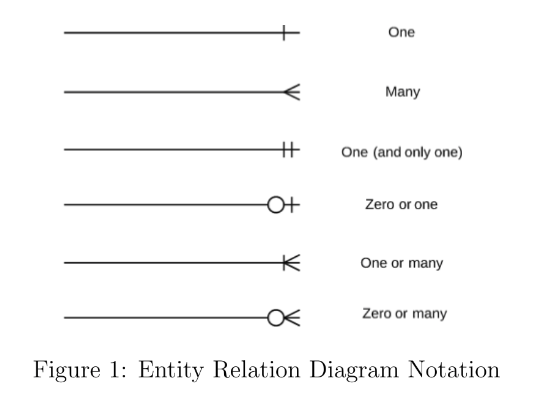
\includegraphics[width=1\textwidth]{ERDNotation} 
    \caption{Entity Relation Diagram Notation}
\end{figure}

Following this notation, our ERD is represented below.

\begin{figure}[H]
    \centering
    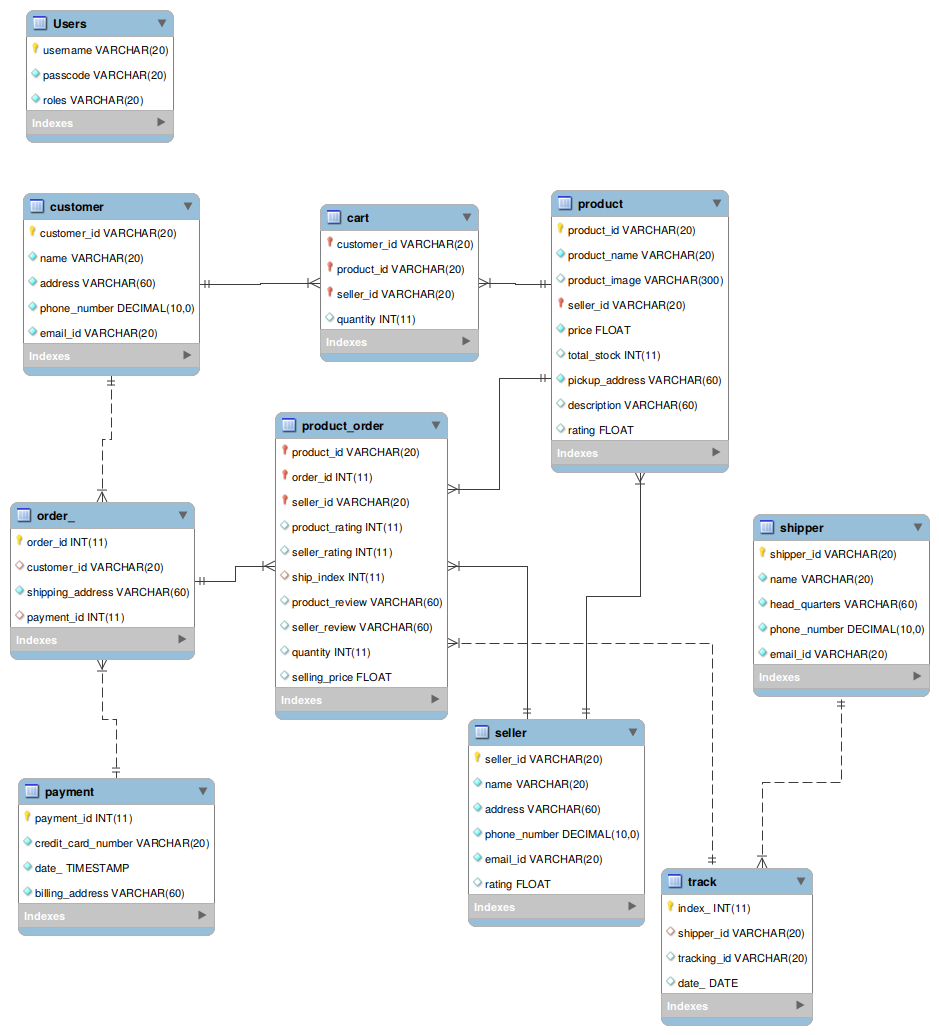
\includegraphics[width=1\textwidth]{ERDL} 
    \caption{Entity Relationship Diagram for e-commerce}
\end{figure}


\section{Database Schema And Normalization}
In this section we describe various aspects of our schema and also mention that it is indeed normalized (BCNF).

\ita{Notation: }A dependency $A \rightarrow B$ is called relevant if all other dependencies from $A$ are of the form $A \rightarrow C$ where $C \subseteq B$.

\begin{itemize}
  \item A table for basic details of customer.
  \begin{minted}{SQL}
/*  Here: customer_id -> R is the only relevant dependency and hence it is in BCNF */
create table customer (
  customer_id VARCHAR (20) primary key not null,
  name VARCHAR (20) not null,
  address VARCHAR (60) not null,
  phone_number DECIMAL (10) UNSIGNED not null,
  email_id VARCHAR (20) not null
);
  \end{minted}
  \item A table for basic details of seller.
  \begin{minted}{SQL}
    /* Here: seller_id -> R is the only relevant dependency and hence it is in BCNF */
    /* Rating will be updated with the help of triggers. */
    create table seller (
      seller_id varchar (20) primary key not null,
      name varchar (20) not null,
      address varchar (60) not null,
      phone_number decimal (10) UNSIGNED NOT NULL,
      email_id VARCHAR (20) not null,
      rating float
    );
  \end{minted}
  \item A table for basic details of shipper.
  \begin{minted}{SQL}
    /*  Here: shipper_id -> R is the only relevant dependency and hence it is in BCNF  */
create table shipper (
  shipper_id varchar (20) primary key not null,
  name varchar (20) not null,
  head_quarters varchar (60) not null,
  phone_number decimal (10) UNSIGNED not null,
  email_id VARCHAR (20) not null
);

  \end{minted}
  \item Having described these basic tables, we can now describe table for products. Note that each product can be sold by different sellers in different price and quantity, thus, primary key is formed by both product\_id and seller\_id. 
  \begin{minted}{SQL}
    /*  Here: (product_id, seller_id) -> R is the only relevant dependency and hence it is in BCNF  */
    /* Rating will be updated with the help of triggers. */
    create table product (
      product_id varchar (20) not null,
      product_name varchar (20) not null,
      seller_id varchar (20) not null,
      price float not NULL,
      total_stock int,
      pickup_address varchar (60) not null,
      description varchar (60),
      rating float,
      foreign key (seller_id) references seller (seller_id) on delete cascade,
      primary key (product_id, seller_id)
    );
  \end{minted}
  \item When user makes a payment, we want to store payment details for which we have the following table.
  \begin{minted}{SQL}
/*   Here: payment_id -> R is the only relevant dependency and hence it is in BCNF  */
create table payment (
  payment_id VARCHAR (20) primary key not null,
  credit_card_number VARCHAR (20) not null,
  date_ timestamp,
  billing_address varchar(60) not null
);
  \end{minted}
  \item User will have a front end feature to add items in cart. When the user is ready to buy, it will generate an \ita{order\_id} for all those products which he or she chose. Note that \ita{order\_id} will be generated \ita{only} when user successfully does the payment.
  \begin{minted}{SQL}
    /* Here: order_id -> R is the only relevant dependency and hence it is in BCNF  */
    create table order_ (
      order_id VARCHAR (20) primary key not null,
      customer_id VARCHAR (20),
      shipping_address varchar(60) not null,
      payment_id VARCHAR (20),
      foreign key (customer_id) references customer (customer_id) on delete set null,
      foreign key (payment_id) references payment (payment_id) on delete set null
    );
  \end{minted}
  \item After generating the payment, we have to put the details of the bought items along with their order\_id.
  \begin{minted}{SQL}
    /*  Here: (product_id, order_id, seller_id) -> R is the only relevant dependency and hence it is in BCNF  */
    create table product_order (
      product_id varchar(20) not null,
      order_id varchar (20) not null,
      seller_id varchar (20),
      product_rating int check (product_rating in (NULL, 1, 2, 3, 4, 5)),
      seller_rating int check (seller_rating in (NULL, 1, 2, 3, 4, 5)),
      ship_index int,
      product_review varchar (60),
      seller_review varchar (60),
      quantity int,
      selling_price float,
      primary key (product_id, order_id, seller_id),
      foreign key (product_id) references product (product_id) on delete cascade,
      foreign key (order_id) references order_ (order_id) on delete cascade,
      foreign key (seller_id) references seller (seller_id) on delete cascade,
      foreign key (ship_index) references track (index_) on delete set null
    );
  \end{minted}
  \item Note that we used a foreign key in the above table which we haven't defined yet, which is \ita{ship\_index}. It is basically a unique identifier for each ordered product serving as an index of track table which we will use to track our items.
  \begin{minted}{SQL}
    /*  Here: index_ -> R is the only relevant dependency and hence it is in BCNF  */
    create table track (
      index_ INT AUTO_INCREMENT primary key not null,
      shipper_id varchar (20),
      tracking_id varchar (20),
      foreign key (shipper_id) references shipper (shipper_id) on delete set null
    );
  \end{minted}
  \item We also have an auxiliary table for keeping track of users with their old passwords as mysql.user encrypts the passwords and there is no way to get it back also this table is required for validation when the user tries to log in the system.
  \begin{minted}{SQL}

-- Clearly this table is in BCNF.
create table Users (
  username VARCHAR (20) primary key not null,
  passcode VARCHAR (20) not null,
  roles VARCHAR (20) not null
);
  \end{minted}
\end{itemize}
\newpage
\section{Roles, Triggers, Views}
\subsection{Views}
\begin{minted}{SQL}
  -- #########################################
-- ###########CUSTOMER VIEWS################
-- #########################################

-- This view will allow customer to view its details.
CREATE VIEW customer_add AS (SELECT * 
                             FROM customer 
                             WHERE CONCAT(customer_id, "@localhost") IN (SELECT user()));

-- This view will allow customer to see the total cost of his/her various orders
CREATE VIEW orderPrice AS (SELECT order_id, sum(selling_price * quantity) as total_price
                           FROM (product_order)
                           GROUP BY order_id); 

-- This view will tell the customer details corresponding to his/her all order_id mentioning complete order details (order_id, shipping_address, date_, total_price) except the products in that order. 
CREATE VIEW previousOrders AS (SELECT T1.order_id, T1.shipping_address, T2.date_, T3.total_price
                               FROM (order_ as T1) NATURAL JOIN (payment as T2) NATURAL JOIN (orderPrice as T3)
                               WHERE CONCAT(T1.customer_id, "@localhost") IN (SELECT user()));

-- This view will allow customer to just see his various order_id. 
CREATE VIEW listOrders AS (SELECT order_id
                            FROM order_ 
                            WHERE CONCAT(customer_id, "@localhost") IN (SELECT user()));

-- This view will give entry to the track table for each (product_id, order_id) pair
CREATE VIEW trackID AS (SELECT order_id, product_id, ship_index
                        FROM product_order
                        WHERE order_id IN (SELECT * FROM listOrders));

-- This view will augment the previous view with tracking_id as well.
CREATE VIEW packageStatus AS (SELECT T1.order_id, T1.product_id, T1.ship_index, T2.tracking_id
                              FROM (trackID as T1) JOIN (track as T2) ON (T1.ship_index = T2.index_));


-- #########################################
-- ###########SELLER VIEWS##################
-- #########################################

-- This view will allow seller to see his/her various products.
CREATE VIEW sellerProducts AS (SELECT product_id, product_name, price, total_stock, pickup_address, description 
                                  FROM product
                                  WHERE CONCAT(seller_id, "@localhost") in (SELECT user()));

-- This view allow seller to see various orders which he or she have sold (seller_id, product_id, quantity, selling_price, date_) 
CREATE VIEW sellerOrders AS (SELECT T1.seller_id, T1.product_id, T1.quantity, T1.selling_price, T2.date_
                                FROM (product_order as T1) natural join (payment as T2)
                                WHERE CONCAT(T1.seller_id, "@localhost") in (SELECT user()));

-- #########################################
-- ###########SHIPPER VIEWS#################
-- #########################################

-- This view will allow shipper details (pickup_address, shipping_address, tracking_id)
CREATE VIEW shipperTrack AS (SELECT index_, pickup_address AS source, shipping_address AS destination, tracking_id
                              FROM (track JOIN product_order ON index_ = ship_index) NATURAL JOIN order_ NATURAL JOIN product 
                              WHERE CONCAT(shipper_id, "@localhost") = (SELECT user()));
\end{minted}

\subsection{Roles}
Basically we have three roles.

\begin{itemize}
    \item A role for database administrator.
    \item A role for customer.
    \item A role for supplier.
    \item A role for shipper.
\end{itemize}

And their details is best understood with the help of the following code:
\begin{minted}{SQL}
  CREATE ROLE dbadmin;
CREATE ROLE customer;
CREATE ROLE seller;
CREATE ROLE shipper;

GRANT ALL PRIVILEGES ON AmaKart.* TO dbadmin;

-- Make sure that any view on which a role gets access on should have the filter "SELECT user()"
GRANT ALL PRIVILEGES ON AmaKart.customer_add TO customer;
GRANT SELECT ON AmaKart.previousOrders TO customer;
GRANT SELECT ON AmaKart.listOrders TO customer;
GRANT SELECT ON AmaKart.packageStatus TO customer;

GRANT SELECT ON AmaKart.sellerProducts TO seller;
GRANT SELECT ON AmaKart.sellerOrders TO seller;

GRANT SELECT ON AmaKart.shipperTrack TO shipper;
\end{minted}

\subsection{Triggers}
\begin{minted}{SQL}
-- When a product is sold, we want to mention its selling_price as later the seller can update the price
DELIMITER //
CREATE TRIGGER setPrice BEFORE INSERT on product_order
FOR EACH ROW BEGIN
  SET NEW.selling_price = (SELECT price FROM product WHERE product_id = NEW.product_id and seller_id = NEW.seller_id);
END//
DELIMITER ;

-- When a customer passes a rating for product we have to update it in our product table
DELIMITER //
CREATE TRIGGER updateRatingProduct AFTER UPDATE on product_order
FOR EACH ROW BEGIN
  IF NEW.product_rating != NULL THEN
    UPDATE product SET rating = (SELECT AVG(product_rating) FROM product_order WHERE product_id = NEW.product_id) WHERE product_id = NEW.product_id;
  END IF;
END//
DELIMITER ;


-- When a customer passes a rating for seller we have to update it in our seller table
DELIMITER //
CREATE TRIGGER updateRatingSeller AFTER UPDATE on product_order
FOR EACH ROW BEGIN
  IF NEW.seller_rating != NULL THEN
    UPDATE seller SET rating = (SELECT AVG(seller_rating) FROM product_order WHERE seller_id = NEW.seller_id) WHERE seller_id = NEW.seller_id;
  END IF;
END//
DELIMITER ;

-- When a product is sold, we need to add an entry to our track table for the same
DELIMITER //
CREATE TRIGGER addTrack BEFORE INSERT on product_order
FOR EACH ROW BEGIN
  INSERT INTO track () Values ();
  SET NEW.ship_index = (SELECT MAX (index_) FROM track);
END//
DELIMITER ;
\end{minted}

\newpage
\section{Functions And Procedures}
Below you can see details description and implementation of various Procedures and Functions

\subsection{Customer Procedures}
\begin{enumerate}
  \item Procedure to see purchases between some duration, "seePurchasesByDate(IN startTime TIMESTAMP, IN endTime TIMESTAMP)" -$>$ Will return complete details from order, payment, product and product\_order table.
  \item Procedure to see items in cart, "getProductsFromCart ()" -$>$ which selects everything from view "showCart".
  \item Procedure for customer to checkout items present in cart, "purchaseEverythingInCart(IN oid varchar(20))" -$>$ which takes in order id and then for each product present in cart, will add the corresponding entry to product\_order table.
  \item Procedure for customer to remove product from cart, "removeProductCart(IN pid varchar(20), IN sid varchar(20))" -$>$ which takes in that products product\_id and seller\_id and thus delete such product from cart (deletion is performed using view showCart).
  \item Procedure for customer to update a product in cart (i.e. change quantity of the chosen product), "CREATE PROCEDURE updateProductCart(IN pid varchar(20), IN sid varchar(20), IN N INT)".
  \item Procedure for customer to make an order, "makeorder(IN cnum varchar(20), IN badd varchar(20), IN cid varchar(20), IN sadd varchar(20))" which takes a credit card number, "cnum", billing address, "badd", customer ID, "cid" and a shipping address, "sadd" and first adds an entry into payment table by selecting date using "NOW()" function and then since payment table had payment\_id which was set to automatic increment so we after fetching it insert the corresponding entries into order\_ table and then again by fetching order\_id as it was auto increment, we call already discussed procedure, "purchaseEverthingInCart".
  \item Procedure to add product to cart, "addProductToCart(IN cid varchar(20), IN pid varchar(20), IN sid varchar(20), IN q int)" which will decide whether to update the quantity if the product is already there in cart, or to add this new record into our cart.
  \item Procedure to see latest N purchases, "seeLatestNPurchases(IN N INT)" which takes in N and then gives rows corresponding to payment, order\_, product\_order, product, table and track (by taking join) ordered decreasingly by payment date.
  \item Procedure to see Purchases between dates, "seePurchasesByDate(IN startTime TIMESTAMP, IN endTime TIMESTAMP)" -$>$ works same as before just that it gives entries between the given time.
  \item Procedure to see products within price range, "queryProductsTim(IN productName varchar(20), IN lowRange FLOAT, IN highRange FLOAT)" -$>$ which after receiving suitable parameters, return entries from product sorted by price between the given range.
  \item Procedure to see reviews of a given product, "ProductReviews(IN pid varchar(20), IN sid varchar(20))" -$>$ will fetch ratings and reviews of the given product from product\_order, etc.
  \item Procedure to add review for a product, "addReviewProduct(IN pid varchar(20), IN oid varchar(20), IN sid varchar(20), IN rev varchar(60))" -$>$ as only those who have purchased successfully the product can add reviews, we need order ID for verification.
  \item Procedure to add review for a seller, "addReviewSeller(IN pid varchar(20), IN oid varchar(20), IN sid varchar(20), IN rev varchar(60))" -$>$ again we need order ID for verification. 
  \item Procedure to add rating for product, "addRatingProduct(IN pid varchar(20), IN oid varchar(20), IN sid varchar(20), IN rating INT)".
  \item Procedure to add rating for seller, "addRatingSeller(IN pid varchar(20), IN oid varchar(20), IN sid varchar(20), IN rating INT)".
  \item Procedure to see products sorted by rating, "queryProductsRat(IN productName varchar(20))".
  \item Procedure to update customer info, custUpdateInfo(IN customer\_id varchar(20), IN password VARCHAR(20), IN name varchar(20), IN address VARCHAR(60), IN phone\_number DECIMAL(10) UNSIGNED, IN email\_id VARCHAR(20)).
\end{enumerate}
\subsection{Seller Procedures}
\begin{enumerate}
  \item Procedure for seller to see sold but not shipped products, soldButNotShipped(IN seller\_id varchar(20)) -$>$ fetches entries from product\_order table which have corresponding shipper\_id NULL.
  \item Procedure for seller to ship a sold product, "shipSoldProduct(IN gproduct\_id varchar(20), IN gorder\_id varchar(20), IN gseller\_id varchar(20), IN gshipper\_id varchar(20), IN gtracking\_id varchar(20), IN gdate DATE)" -$>$ will ship the product (update shipper\_id and tracking\_id in track table) by taking relevant input.
  \item Procedure for seller to see his rating, "getRating(IN seller\_id varchar(20))".
  \item Procedure for seller to check whether there is already a product with given seller\_id and product\_id (this is useful when seller is adding a new product), "sellerCheckExistProd(IN product\_id varchar(20), IN seller\_id varchar(20))" -$>$ will return a row if there is a corresponding product.
  \item Procedure for seller to add new product, "addProduct(IN product\_id varchar(20), IN seller\_id varchar(20), IN product\_name varchar(20), IN product\_image varchar(300), IN price float, IN total\_stock int, IN pickup\_address varchar(60), IN description varchar(60))" -$>$ adds an entry in product table by taking suitable input details.
  \item Procedure for seller to update his specific product details, "updateProductInfo(IN product\_id varchar(20), IN seller\_id varchar(20), IN product\_name varchar(20), IN product\_image varchar(300), IN price float, IN total\_stock int, IN pickup\_address varchar(60), IN description varchar(60))" -$>$ Note that it is possible to call this procedure by giving empty string for entries whose update is not deemed fit.
  \item Procedure to update seller's info, "sellerUpdateInfo(IN seller\_id varchar(20), IN passwordd VARCHAR(20), IN named varchar(20), IN addressd VARCHAR(60), IN phone\_number DECIMAL(10) UNSIGNED, IN email\_id VARCHAR(20))" -$>$ Note that it is possible to call this procedure by giving empty string for entries whose update is not deemed fit.
  \item Procedure for seller to see his or her past sold products within a specific time duration, "seeSellingsBetweenDuration(IN startTime TIMESTAMP, IN endTime TIMESTAMP)" -$>$ fetches the relevant entries from product\_order table.
  \item Procedure to see latest N sellings, "seeLatestNSellings(IN N INT)" -$>$ fetches the relevant entries from product\_order table.
  \item Procedure to see seller's already listed similar products with increasing price, "selQuerySimProducts(IN productName varchar(20))".
  \item Procedure to see seller's similar products sorted by rating, "selQueryProductsRat(IN productName varchar(20))".
\end{enumerate}
\begin{minted}{SQL}
  -- #########################################
  -- ###########SHIPPER PROCEDURES############
  -- #########################################
  
  
  
  -- Procedure to update shipper's info
  DELIMITER //
  CREATE PROCEDURE shipperUpdateInfo(IN shipper_id varchar(20), IN passwordd VARCHAR(20), IN named varchar(20), IN addressd VARCHAR(60), IN phone_number DECIMAL(10) UNSIGNED, IN email_id VARCHAR(20))
  BEGIN
      IF (CHAR_LENGTH(passwordd) > 0) THEN
        UPDATE Users SET Users.passcode = passwordd WHERE Users.username = shipper_id;
      END IF;
      IF (CHAR_LENGTH(named) > 0) THEN
        UPDATE shipper SET shipper.name = named WHERE shipper.shipper_id = shipper_id;
      END IF;
      IF (CHAR_LENGTH(addressd) > 0) THEN
        UPDATE shipper SET shipper.head_quarters = addressd WHERE shipper.shipper_id = shipper_id;
      END IF;
      IF (phone_number <> 0) THEN
        UPDATE shipper SET shipper.phone_number = phone_number WHERE shipper.shipper_id = shipper_id;
      END IF;
      IF (CHAR_LENGTH(email_id) > 0) THEN
        UPDATE shipper SET shipper.email_id = email_id WHERE shipper.shipper_id = shipper_id;
      END IF;
  END;
  //
  DELIMITER ;
  
  -- Procedure for shipper to see his or her past shipments within a specific time duration
  DELIMITER //
  CREATE PROCEDURE seeShipmentsBetweenDuration(IN startTime DATE, IN endTime DATE)
  BEGIN
      select * from track where CONCAT(shipper_id, "@localhost") IN (SELECT user()) AND date_ BETWEEN startTime AND endTime;
  END;
  //
  DELIMITER ;
  
  -- Procedure to see latest N Shipments
  DELIMITER //
  CREATE PROCEDURE seeLatestNShipments(IN N INT)
  BEGIN
      select * from track where CONCAT(shipper_id, "@localhost") IN (SELECT user()) ORDER BY date_ DESC LIMIT N;
  END;
  //
  DELIMITER ;
  
  -- #########################################
  -- ################FUNCTIONS################
  -- #########################################
  
  -- Function to return the total earning of a seller between supplied dates
  DELIMITER //
  CREATE FUNCTION sellerStatsBetweenDate(startTime TIMESTAMP, endTime TIMESTAMP)
  RETURNS FLOAT DETERMINISTIC  
  BEGIN
      DECLARE temp FLOAT;
      SELECT SUM(quantity*selling_price) INTO temp FROM product_order natural join order_ natural join payment WHERE date_ BETWEEN startTime and endTime;
      RETURN temp;
  END;
  //
  DELIMITER ;  
\end{minted}
\section{Use Cases}
Lets for this case assume that we a supplier. We first want to register and then add products to sell.
\begin{figure}[H]
    \centering
    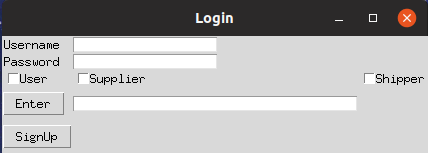
\includegraphics[scale=0.5]{login1.png} 
    \caption{Login page.}
\end{figure}
So at the login page we will select SignUp. It will then open up the SignUp page.
\begin{figure}[H]
    \centering
    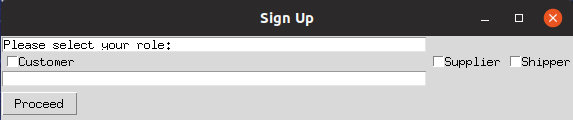
\includegraphics[scale=0.5]{signup1.png}
    \caption{SignUp page(Selecting role).}
\end{figure}
Since we are Supplier we will select supplier option and then proceed.
\begin{figure}[H]
    \centering
    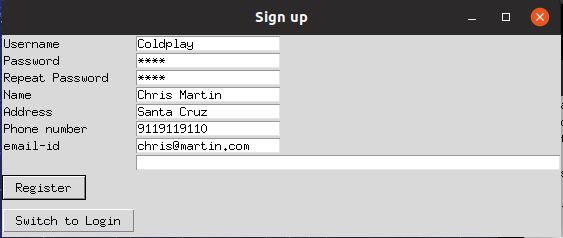
\includegraphics[scale=0.5]{signup2.png}
    \caption{SignUp page(Entering Details).}
\end{figure}
After entering the details press the Register button. It will display that the user is successfully created.
\begin{figure}[H]
    \centering
    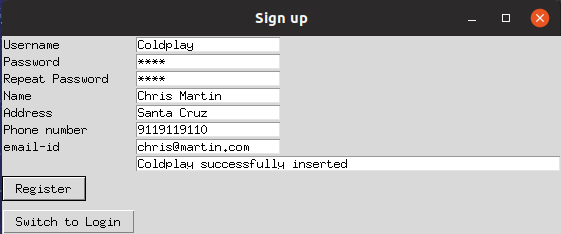
\includegraphics[scale=0.5]{signup3.png}
    \caption{SignUp page(Conformation).}
\end{figure}
After registering goto the login page by pressing the Switch to Login button.
\begin{figure}[H]
    \centering
    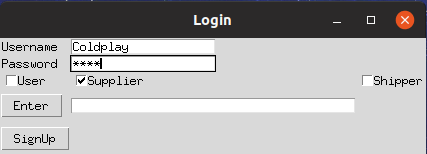
\includegraphics[scale=0.5]{login2.png} 
    \caption{Login page(Entering Details).}
\end{figure}
After login you will be taken to a welcome page which will have two options for you 
\begin{itemize}
    \item Either to add new products in the market.
    \item Or to change the quantites or price of existing products. 
\end{itemize}
\begin{figure}[H]
    \centering
    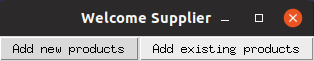
\includegraphics[scale=0.5]{supp1.png} 
    \caption{Welcome page for Supplier.}
\end{figure}
So lets add a new product. You will be taken to a page which will ask to fill the details of the product.
\begin{figure}[H]
    \centering
    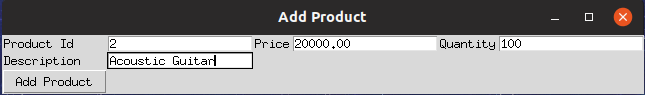
\includegraphics[scale=0.5]{supp2.png} 
    \caption{Add new product.}
\end{figure}
Now the product has been added successfully.

\newpage
\section{Progress And TODOS}
\subsection{GUI}
\begin{itemize}
  \item Signup is working perfectly (just that inplace of integer if string is given then its an issue, can write a function to check it though).
  \item Login is working perfectly.
  \item 
\end{itemize}
\section{Useful links}
\begin{center}
\textbf{Complete project - } \href{https://github.com/nikhilyadv/DBMS-Lab-Project}{Link}\\
\textbf{GUI source code - } \href{https://github.com/nikhilyadv/DBMS-Lab-Project/tree/master/GUI}{Link}
\end{center}
\end{document}